% 来源：OEBPS/Text/Section0001_split_007.xhtml#sigil_toc_id_51

\BookChapter{38}
\section[第38章\q 玛丽·卡拉汉·厄道斯：管理万亿美元资产的女人]{第38章\\ 玛丽·卡拉汉·厄道斯：管理万亿美元资产的女人}

\begin{figure}[htbp]
\centering
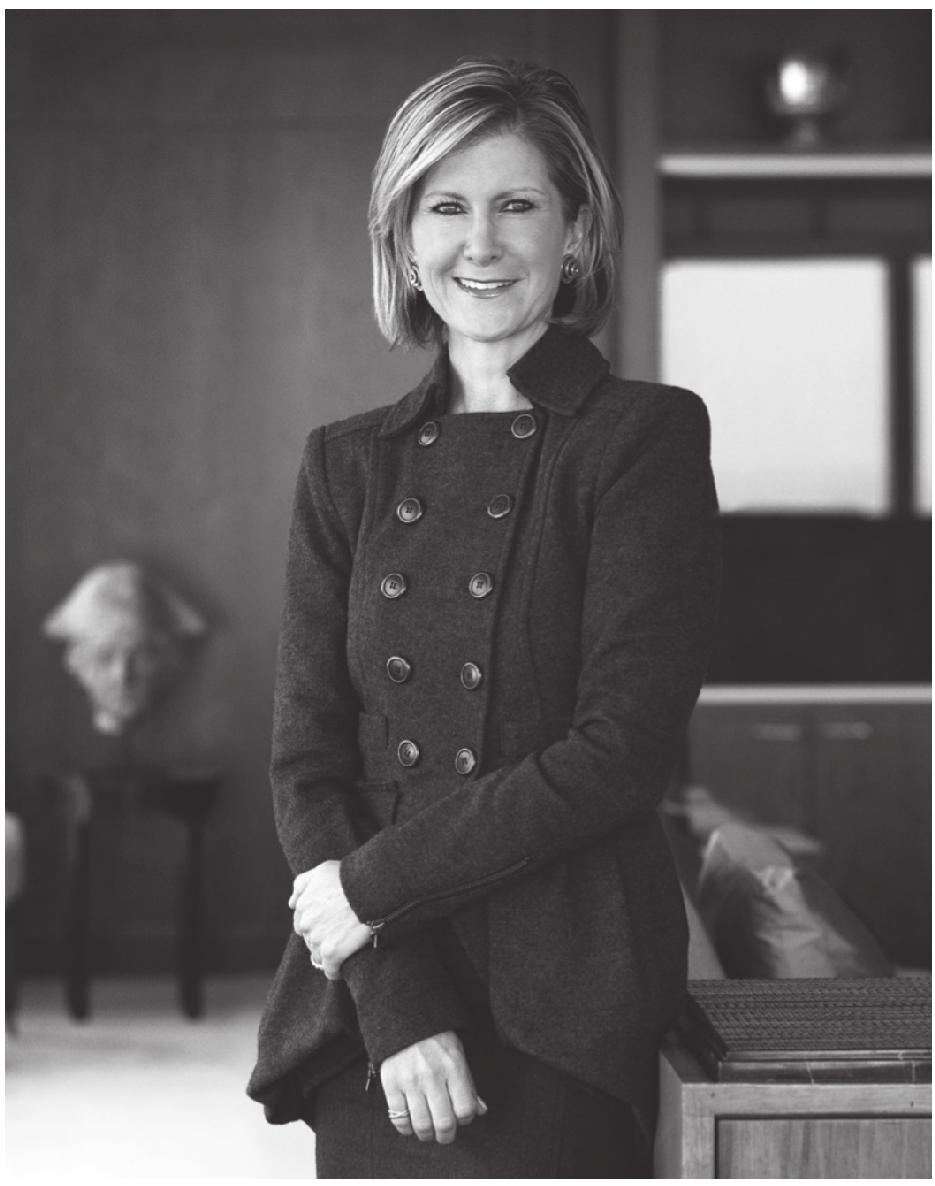
\includegraphics[width=0.42\linewidth,keepaspectratio]{image/玛丽·卡拉汉·厄道斯肖像.jpg}
\caption*{玛丽·卡拉汉·厄道斯}
\end{figure}

摩根大通资产管理集团首席执行官

玛丽·卡拉汉·厄道斯可能不到1米56，这位身材娇小的女士，影响可不小，她担任世界上最大的资产管理集团摩根大通资产管理集团的首席执行官。摩根大通集团是美国最大的银行之一。《福布斯》杂志称厄道斯为“在男性主导的华尔街企业里非常罕见的女强人”，而且评选她为“世界上100位最有影响力的女人”之一。从2009年厄道斯接管摩根大通资产管理集团以来，资产管理规模增加接近5000亿美元，增幅超过30\%。厄道斯监督管理的资产规模达到2.5万亿美元，服务的投资人包括基金会、各国中央银行、养老基金，还有一些世界上最富有的人。媒体经常把她列为接替摩根大通首席执行官杰米·戴蒙的少数候选人之一。

尽管在本书访问的50多位投资理财超级明星中，大多数人都赞同投资指数基金，采取这种被动的、低费率的资金管理方式，长期来看，能够为个人投资者带来最好的业绩，可是厄道斯说，行业内最优秀的基金经理做主动管理型的基金所创造的业绩更好，和他们收取的费用相比，物超所值。她说，证据就摆在那里，这些优秀基金经理人的客户非常忠诚，长期持有基金，而且这些基金经理继续吸引新的资金进来，管理规模不断扩大。

资金管理从小就融入厄道斯的血液里了。她出生在温尼卡一个爱尔兰天主教大家庭，她是家里的第一个出生的孩子，也是唯一的一个女孩子，他的父亲帕特里克·卡拉汉是个投资银行家，在芝加哥的拉扎德公司工作。厄道斯在读高中的时候数学成绩就非常突出，还赢得了马术比赛的奖牌，后来她读了乔治城大学，成为他们那届数学专业中唯一一名女学生。后来，她在哈佛大学商学院读工商管理硕士时遇到了她的丈夫菲利普·厄道斯。

作为一名金融服务行业的高管，厄道斯在很多方面打破了原有的模式：这个行业以侵略性管理而闻名，非常男性化，而她的同事用这样的词语来描述她：“忠诚”“团队为先”“有爱心”。厄道斯在摩根大通一路奋斗，晋升到最高管理层。她最有名的就是在服务客户上非常投入，她经常飞越整个美国去见客户，给客户在管理资产上提供额外的帮助。她47岁，成为这个有2.6万名员工的公司的最高管理人。她受人尊敬，一是因为她投资理财的专业能力很强，二是因为她的领导能力卓越非凡。

我们俩的会面就在摩根大通的全球总部，那座古典的联合碳化大楼里，那里可以俯瞰派克大街和曼哈顿的摩天大楼。我坐上电梯前往会议室，摩根大通资产管理集团的公关部主管达林·奥多约讲了一个她自己的故事，深深触动了我，从中也可以看出，我要见的这位首席执行官是个什么样的人。奥多约一直想当节目主持人，却在摩根大通的公募基金部门找到了工作。后来能转到公关部门，还是厄道斯的功劳。厄道斯让奥多约去当制片人，做一档晨间会议广播，播放给财富管理集团全球2万多名同事，他一听就惊呆了。

“我对投资知道得不够多！”奥多约反对说。

“是你告诉我，你一直想当一个节目主持人。”厄道斯说，“现在你要更上一层楼，成为一个谈话节目的制片人。”

“她看我看得很透，比我自己看自己还要透。”奥多约告诉我。

不管这些员工在公司做的是什么工作，厄道斯都用自己的方式，尽可能多地了解他们。此外，她还尽量想方设法地留出固定的时间，和她的三个小女儿共进午餐，开车送她们上学，大多数日子都是这样的。这是厄道斯这位母亲的方式，这种方式既让她成为非凡的企业领导者，又让她做好一个普通人——她就是这样独特。

\begin{BookQuote}
\textbf{罗宾斯：}你领导着世界上规模最大的资产管理集团，请问你是怎么一路走过来的？你面对过什么样的挑战？指导你的基本原则是什么？
\end{BookQuote}

\begin{BookQuote}
\textbf{厄道斯：}我想，你不可能精确地规划出人生要走的路，正好能让你到达你想去的地方，很多事情发生了，有的靠运气，有的是环境的关系。
\end{BookQuote}

我还记得我得到的第一只股票——联合碳化，这是我奶奶送给我的生日礼物。我那时有七八岁吧，那个年纪开始记事了，但是毕竟还很小，我不知道拿这股票该怎么办。

我奶奶告诉我的第一件事情是：“这个股票不能卖掉。”当时我不敢肯定我能不能做到，但是我奶奶说：“这就是复利的价值，如果你一直拿着这只股票，那么这只股票就有希望随着时间的推移不断地增值，最后你得到的价值要比现在大得多。”奶奶这番话，在七八岁的我的心里种下了投资的种子，让我知道了储蓄的重要性，让我开始思考资金管理。当时我已经感觉到我对数字很敏感，对于我来说存钱比花钱的概念更强大有力。

正好我父亲也在金融行业工作，这对我很有帮助，有很多周末他在办公室加班，我就陪着他在办公室“玩”，我坐他的办公桌，让我的几个小弟弟坐他助理的办公桌，我当然是大姐大啦！我们就这样在陪着爸爸加班中长大，很有乐趣。我想，这让我觉得金融服务业多么有趣好玩，又多么让人兴奋激动，它不是什么让你恐惧害怕的东西。在我人生的早期阶段，这种感觉对我很有帮助。

\begin{BookQuote}
\textbf{罗宾斯：}你所在的金融行业，一直都是男性做主导。这一路走过来，你面对了哪些最大的挑战？
\end{BookQuote}

\begin{BookQuote}
\textbf{厄道斯：}资金管理这个行业，用业绩说话。实际上这是个循环：你给客户管理资金的业绩好，他们就会投入更多的钱让你管理，他们投入更多的钱，你就会赚更多的钱。这就是我从我奶奶那里学到的复利的巨大作用。因为专注于业绩，资金管理这个行业更容易形成男女平等。你只要业绩表现好，就会成功。
\end{BookQuote}

\begin{BookQuote}
\textbf{罗宾斯：}什么是领导力？你怎么定义领导力？
\end{BookQuote}

\begin{BookQuote}
\textbf{厄道斯：}不要把管理和领导搞混，这一点很重要。我的看法是，管理是我自己不愿意做的事，也不要让任何人去做。领导就是每天早上醒来，努力让你领导的这个组织变得比以前更好，我真的相信，我是为了摩根大通资产管理集团的人工作的，而不是让大家为我工作。正是因为这个原因，我要努力比大家看自己还要看得更高更远。
\end{BookQuote}

我做过投资组合经理、客户顾问、企业领导者，我知道，我们能够为客户取得什么样的成就，所以我觉得我的工作并不是领导我们的团队，而是钻到战壕里，与团队一道战斗，与团队一路同行，我认为，从很多方面来说，你要么天生有领导力，要么就没有，但这并不意味着你不能。持续不断地修炼，持续不断地精进，搞清楚什么领导方法有效、什么无效。领导的风格要随着不同的人、不同的环境而有所改变，但是领导的基本原则是一直不变的。

\begin{BookQuote}
\textbf{罗宾斯：}最近我访问了罗伯特·席勒博士，他曾赢得诺贝尔经济学奖，他谈到金融机构在这个世界上做的所有好事，人们都以为那是理所当然的。你认为金融机构的名声是不是已经变差了？能做些什么来恢复金融机构的声誉？
\end{BookQuote}

\begin{BookQuote}
\textbf{厄道斯：}因为发生了金融危机，所以这可以理解，为什么有些人对金融行业失去了信心。回过头来看，确实有些事情需要改变，有些产品太复杂，太容易让人困惑。但是总体来说，金融服务行业对这个世界做出了很大贡献。我们为公司提供成长所需要的资本，最终推动了就业增长。我们帮助个人把他们辛辛苦苦赚来的钱储蓄起来，去做投资，赚更多的钱，让他们有钱去做自己想做的事，例如买房子、付大学学费、退休后能过上舒服的晚年生活，我们支持当地的社区发展，在金融上支持，也用我的智力资本和物质资本积极支持。
\end{BookQuote}

我非常骄傲能加入金融行业，我也更加骄傲能够加入摩根大通资产管理集团。我们有2.6万名员工，每天努力工作，为客户提供服务，总是尽力做正确的事。我们有个说法是，如果你不愿意让奶奶买这个产品，那么这个业务我们就不应该做。这种看问题的方法非常简单，但是非常重要。

\begin{BookQuote}
\textbf{罗宾斯：}有个敏感的话题。我可以肯定，如果你问瑞·达利欧、约翰·博格、戴维·斯文森、沃伦·巴菲特，他们都会说主动管理型投资长期而言无法战胜市场。96\%的主动管理型基金经理无法战胜指数，我想听听你对这个问题的看法，因为你的投资业绩一直非常出色。
\end{BookQuote}

\begin{BookQuote}
\textbf{厄道斯：}成功投资面临的最大困难是，没有一个包治百病的万能投资方式，但是如果你看看世界上最成功的投资组合经理，你会发现，他们很多人都是积极主动地管理资金，买进和卖出他们觉得自己比市场看得更加清楚、更加明白的公司股票。他们的历史业绩记录已经证明了主动管理型资金经过长期的复利，可以让你的投资组合业绩有极大的不同。主动管理型基金经理能够做的就是，分析两个看起来非常相似的公司，根据深入研究做出判断，哪个才是更好的长期投资。在摩根大通资产管理集团，我们身边有好多基金经理，在较长的一段时间内，他们都做得相当成功，这也正是为什么客户会让我们来帮助管理2.5万亿美元的资产。
\end{BookQuote}

\begin{BookQuote}
\textbf{罗宾斯：}伟大的投资者几乎总是在寻找风险—收益不对称的投资机会，对不对？那些超级富豪一直在做这样的事。请问，普通的投资者现在如何能够获得财富又不用承担风险，或者至少是获得财富而只承担很小的风险，如果他们现在不是超级富有的话？
\end{BookQuote}

\begin{BookQuote}
\textbf{厄道斯：}这件事和财富水平没有关系，关键是你要有周密的准备，能够得到良好的投资建议，然后一直坚持你的投资计划。经常发生的情况是，他们刚开始也是按照计划做分散投资，但是随着市场情况的变化，他们就开始想要预测市场的未来走势，要么是行情上涨的时候想抓住更多上涨的机会，要么是在行情下跌相当不利的情况下想要更好地保护自己，结果偏离了原来分散投资的计划。但是这样预测市场走势、择时交易是非常危险的，因为你根本不可能准确地预测到每一种情境。
\end{BookQuote}

一个做到良好分散投资的组合，能帮助你俘获那些尾部风险，这些风险不大，但是能够带来巨大回报。你如果坚持原来的计划，长期而言，就能创造出数量巨大的财富。

\begin{BookQuote}
\textbf{罗宾斯：}今天的投资者最大的投资机会有哪些？最大的挑战又有哪些？他们需要做好什么准备？
\end{BookQuote}

\begin{BookQuote}
\textbf{厄道斯：}我想，将来我们回头看现在，肯定会说：“那是一个应该投资的绝好时机。”我们现在这个经济体系流动性很大，可以解决很多过去的错误。但是，现在是个5年投资的好机会，特别是那些有长期增长前景的投资项目。很多投资者现在只想要稳定的收入，温和的波动性、流动性。这是由于2008年金融危机的影响还在心头萦绕，很多人非常担心：“如果我现在就需要钱，我能拿到钱吗？”如果你并不是现在就需要钱，就拿这些钱去投资吧。你的这些投资，未来5\textasciitilde{}10年会给你带来丰厚的回报。到时候回头看，你会非常庆幸自己实在是英明果断。
\end{BookQuote}

此外，金融行业在法律法规上做出了很多改变，努力保证未来有更好的投资环境。这并不是说，以后就不会有异常巨大的市场波动，但是整个市场体系更好，所以也应该会更安全。

\begin{BookQuote}
\textbf{罗宾斯：}每一次和白手起家，后来赚到几十亿财富的超级富豪交流，我都会问他这个问题：有了几十亿财富，财务压力是不是从此离你而去了？
\end{BookQuote}

\begin{BookQuote}
\textbf{厄道斯：}财务压力永远不会离去，不管你有多么巨大的财富，不管你取得多大的成功。
\end{BookQuote}

\begin{BookQuote}
\textbf{罗宾斯：}怎么会这样？
\end{BookQuote}

\begin{BookQuote}
\textbf{厄道斯：}不管你处于什么人生阶段、什么财富水平，你都想确定你是在最高效地使用你的钱，不管你是花钱做医疗保健，还是花钱让家人生活得更好，或者你想确保你的钱做的长期投资是合适的，能够满足将来子孙后代的需要，或者能够实现你的慈善捐赠目标。
\end{BookQuote}

\begin{BookQuote}
\textbf{罗宾斯：}这种财务压力有没有什么解药？你碰到财务压力时如何缓解？
\end{BookQuote}

\begin{BookQuote}
\textbf{厄道斯：}我自己缓解心理上的财务压力，关键在于正确恰当地处理问题，集中关注那些你能够控制的事情，比如确保每一天你能做多少就尽可能地做多少，你能给予多少就尽可能地给予多少。千万不要失去平衡，照顾好你自己，做个完整的人；照顾好你的工作，做个优秀的专业人士；照顾好你的家庭；照顾好你的朋友；照顾好你的头脑；照顾好你的身体。每隔一段时间，肯定会有些事情偏离正轨，这很正常，但是如果它们一直偏离正轨，那就不正常了。
\end{BookQuote}

\begin{BookQuote}
\textbf{罗宾斯：}如果你一分钱都不能留给孩子，只能留给他们一套规则，或者一套投资组合策略，或者一个资产配置策略，那么它会是什么？
\end{BookQuote}

\begin{BookQuote}
\textbf{厄道斯：}长期投资，一直持有很多年，只有你真的需要钱的时候，才卖出一些投资，够用就行了。具体构建什么样的投资组合，因人而异。例如，我有三个女儿，三个人年纪不同、技能也各有不同，而且随着时间变化，她们也会发生变化。有的人花钱可能更多一些；有的人可能更加节俭。有的人要找个好工作，想让自己赚很多钱；有的人可能天性喜欢做慈善。有的人可能结婚；有的人可能不愿意结婚。有的人会要孩子，有的人可能不愿意要孩子。总之，她们会有很多不同的地方，相当于方程式有很多不同的变量。每一个单独的变量，都会随着时间的推移而改变，这正是为什么从她们出生的第一天起，我就给每个孩子分别设立了一个投资组合，每个人的投资组合会随着时间的推移而改变。
\end{BookQuote}

\begin{BookQuote}
\textbf{罗宾斯：}你的孩子们多大了？
\end{BookQuote}

\begin{BookQuote}
\textbf{厄道斯：}11岁，10岁，7岁。她们都很有意思。
\end{BookQuote}

\begin{BookQuote}
\textbf{罗宾斯：}我读了很多关于你的采访报道，按照我的理解，你相信“工作生活合二为一”。能给我们更加详细地解释一下吗？
\end{BookQuote}

\begin{BookQuote}
\textbf{厄道斯：}我真是非常幸运，能够在摩根大通这样一家公司工作，因为公司对员工的家庭非常支持，给了员工很多的灵活性，可以选择对自己最好的方式来安排好工作和生活。这意味着你可以早点儿下班，去看孩子的足球比赛，但是比赛完了你会重新回到公司，晚上加班，直到你的工作任务完成。或者周末把你的孩子带到办公室，一边加班一边陪着孩子，两不耽误，就像我小时候父亲周末带着我去办公室加班一样，我们都有一些工作上的选择和安排，可以去做对你和你的家庭最好的事情，同时也不会耽误你及时完成工作。
\end{BookQuote}

\begin{BookQuote}
\textbf{罗宾斯：}哈哈，你的孩子就像你小时候坐在你父亲办公室里一样！孩子坐在你的办公桌后面，为未来做好准备。
\end{BookQuote}

\begin{BookQuote}
\textbf{厄道斯：}对，我的工作和家庭生活，其实都是一回事，都是我的生活，都是我的人生，我总是决心要做到工作和家庭都要好，这才是我想要的最美好的人生。
\end{BookQuote}
